\section{Definicje}

\begin{definition}
    Mówimy, że maszyna M (deterministyczna lub nie) \textbf{działa w czasie} \( T : \natural \rightarrow \natural \) jeśli dla każdej konfiguracji startowej \( q_0 w \) każde obliczenie jest akceptujące lub odrzucające i ma długość co najwyżej \( T(\abs{w}) \)
\end{definition}

\begin{definition}
    Język \( L \) jest w klasie P (polynomial) jeśli istnieje wielomian \( p \)
    oraz Deterministyczna Maszyna Turinga działająca w czasie \( p \) taka, że \( L(M) = L \)
\end{definition}

\begin{definition}
    Język \( L \) jest w klasie NP (nondeterministic polynomial) jeśli istnieje wielomian \( p \) oraz Niedeterministyczna Maszyna Turinga działająca w czasie \( p \).
\end{definition}

\begin{definition}
    \( \textsc{PTIME} = \bigcup_{k=0}^\infty \textsc{TIME}(n^k) \)
\end{definition}

\begin{definition}
    \( \textsc{NPTIME} = \bigcup_{k=0}^\infty \textsc{NTIME}(n^k) \)
\end{definition}


\begin{definition}
    Mówimy, że funkcja \( f \) jest \textbf{redukcją wielomianową} jeśli istnieje wielomian \( p \) oraz Maszyna Turinga obliczająca \( f \) w czasie \( p \). 
    
    Jeśli istnieje redukcja wielomianowa z języka \( L_1 \) do języka \( L_2 \) to zapisujemy to jako \( L_1 \leq_p L_2 \)
\end{definition}

\begin{definition}
    Problem \( L \) jest \textbf{NP-trudny} jeśli \( \forall_{L' \in NP} L' \leq_p L \)
\end{definition}
\begin{definition}
    Problem \( L \) jest \textbf{NP-zupełny} jeśli jest NP-trudny i \( L \in NP \)
\end{definition}

\begin{lemma}
    Jeśli \( L \) jest NP-trudny i \( L \leq_p L' \) to \( L' \) jest NP-trudny. 
\end{lemma}



\section{SAT}

\begin{definition}
    Problem spełnialności boolowskiej SAT\footnote{Na wykładzie nazywany PSB, dla odróżnienia od CNF-SATa} dostaje na wejściu formułę rachunku zdań \( \varphi \) a na wyjściu odpowiada ''TAK'' jeśli istnieje wartościowanie \( v: X \rightarrow \set{0, 1} \) które spełnia tę formułę.
\end{definition}

\begin{theorem}[Cook-Levin]
    Problem \( SAT \) jest NP-zupełny
\end{theorem}
\begin{proof}
    Oczywiście \(SAT \in NP\) bo możemy ''zgadnąć'' wartościowanie.
    
    Pokażemy, że SAT jest NP-trudny.
    
    W tym celu musimy pokazać, że jeśli \( L \in NP \) to istnieje redukcja z \( L \) do \( SAT \).
    Skoro \( L \in NP \) to istnieje MT \( M \), która go akceptuje. 
    
    Intuicyjnie -- będziemy śledzić obliczenie prowadzone przez \( M \) na zadanym słowie wejściowym \( w \) i zapisywać je jako formułę logiczną.
    
    \( M \) działa w czasie \( p(\abs{x}) \) zatem możemy wyobrazić sobie tablicę o wymiarach \( p(\abs{x}) \times p(\abs{x}) \) w której wiersze reprezentują kolejne konfiguracje maszyny.

    Możemy skonstruować formułę logiczną która będzie opisywała jakie są poprawne przejścia w konfiguracjach maszyny.
    
    W formule będą występować zmienne \( X_{i, a, t} \) które będą oznaczać, że ''w \( t \)-tym kroku maszyny \( i \)-ta komórka na taśmie miała wartość \( a \)''.
\end{proof}


\section{3-kolorowanie}
SAT jest bardzo fajnym problemem, bo pokazuje że mamy jakiś problem NP-zupełny i jest to dobry punkt wyjścia do pokazywania, że inne problemy są NP-zupełne.

\begin{definition}
    Instancją problemu 3-kolorowania definiujemy następująco:
    \begin{enumerate}
        \item IN: Graf G = (V,E)
        \item PYTANIE: Czy G jest 3-kolorowalny, tzn. czy istnieje funkcja \(c : V \rightarrow \set{1, 2, 3} \) taka, że \[
            \forall_{(u, v) \in E} : c(u) \neq c(v) 
        \]
    \end{enumerate}
\end{definition}

\begin{theorem}
    3-COL jest \np-zupełny.
\end{theorem}
\begin{proof}
    Na początku należy udowodnić, że problem ten należy do \np. Jest to oczywiste: możemy stworzyć NMT zgadującą kolorowanie grafu, a następnie weryfikującą poprawność kolorowania w czasie wielomianowym.
    
    Teraz musimy udowodnić, że ten problem jest \np-trudny. Korzystamy z faktu, że 3-SAT jest \np-trudny\footnote{Dowód pomijamy, bo zadanie to było na ćwiczeniach.}. Dla każdej formuły $\varphi$ w 3-CNF musimy wobec tego znaleźć algorytm wielomianowy taki, że 3-CNF jest spełnialna wtw gdy $G(\varphi)$ jest 3-kolorowalny. 
    
    \begin{equation*}
        \varphi = \bigwedge_{i=1}^m (l_i^1 \lor l_i^2 \lor l_i^3) 
    \end{equation*}
    
    Wprowadzamy globalny gadżet, który będzie przepisywał kolorom wartości prawda/fałsz.
    
    \begin{figure}[H]
        \centering
        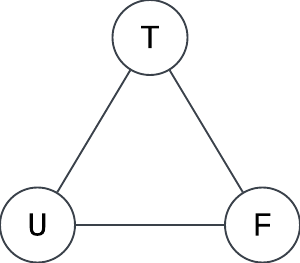
\includegraphics{img/3-coloring-global-gadget.png}
        \caption{Gadżet globalny -- T odpowiada prawdzie, F fałszowi, a U sztucznemu stanowi}
    \end{figure}
    
    Dla każdej zmiennej $x_i$ wprowadzamy gadżet, tworząc też graf $G(\varphi) = (V(\varphi), E(\varphi)$. Gadżet ten wygląda tak, że mamy 2 wierzchołki, jeden o nazwie $x_i$, drugi $~x_i$ (i krawędź między tymi dwoma wierzchołkami).
    
    \begin{figure}[H]
        \centering
        
\includegraphics{img/3-coloring-variable-gadget.png}
        \caption{Gadżet dla zmiennej \( x \)}
    \end{figure}
    
    Dla każdej klauzuli wprowadzamy gadżet $\psi $, który jest definiowany dla każdej klauzuli z osobna. Jest to taki dziwny dzyndzek, który ma trzy początki i którego każdy początek utożsamiamy z jedną zmienną. Semantycznie ma to tworzyć pewnego rodzaju bramkę OR. Teraz udowodnimy, że jeśli ten graf ma 3-kolorowanie to formuła jest spełnialna. 
    
    \begin{figure}[H]
        \centering
        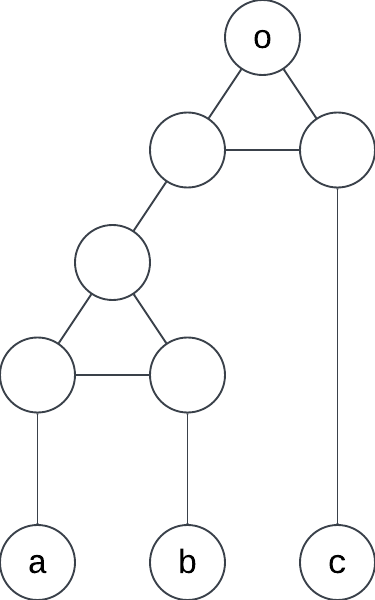
\includegraphics{img/3-coloring-clause-gadget.png}
        \caption{Gadżet dla klauzuli \((a \lor b \lor c) \)}
    \end{figure}
    
    Wierzchołki \( a , b, c \) są wierzchołkami literałów (z poprzedniego kroku), a wierzchołek \( o \) łączymy z wierzchołkami \( F \) i \( U \) (wtedy musi dostać kolor taki jak \( T \))
    
    Wykonujemy super obserwację: Każde poprawne 3-kolorowanie $k$ gadżetu \(C\psi\) (kolorami o nazwach T,F i U) spełnia \(\{c(l_i^1), c(l_i^2), c(l_i^3)\} = t\) jeśli \(k(F) = 1\) i \(c(v) = v\). 
    
    Wynika to z tego, że \(c(F) = f\), \(c(u) = u\), \(c(T) = t, c(v_6) = t, c(v_4) = f \lor c(v_5) = t \).
        
    Następnie dowodzimy, że jeśli \( \varphi\) jest spełnialna to graf jest 3-kolorowalny.
    
    Następnie, że jeśli graf ma 3-kolorowanie to \( \varphi \) jest spełnialna: nasz trójkąt ma 3 wierzchołki które nazwaliśmy \(T, F, U\). \(U\) to było to co się łączyło z oboma końcami zmiennych, \(F\) z końcami gadżetów. No i odzyskujemy wartościowanie formuły z grafu, zależnie od tego jaki kolor dostały (nazwy kolorów utożsamiamy z tym jakie kolory dostał← na trójkącie jakby). 
    
    No i dowodzimy że to jest redukcja wielomianowa, ale to widać w miarę, bo ten graf jest jakiś rozmiaru \(\mathcal{O}(\varphi)\). (coś tam coś tam machu machu)
    
\end{proof}

Pamiętajmy, że jak mówimy o dopełnieniach problemów to nie mówimy o dopełnieniu do \( \Sigma^* \) per se, bo są kodowania które są głupie i ich nie rozpatrujemy. 

Śmieszne pytanie: czy \np jest zamknięte na dopełnienie? Czy \(P\) jest zamknięte na dopełnienie? Dla \(P\) wystarczy po prostu zamienić stan akceptujący na odrzucający i vice versa.

Dla \np nasz sprytny plan się pierniczy, bo niedeterministyczne maszyny Turinga mówią że akceptują x jeśli \textit{istnieje} obliczenie akceptujące: jeśli zmienimy stany to nam to nie da dopełnienia problemu, a jakieś trochę takie bzdury. 

I niestety okazuje się, że ludzkość nie zna odpowiedzi na to pytanie (whoopsie). 

\begin{definition}
     \(  L \in  \conp \iff L^C  \in \np \).
\end{definition}

\begin{definition}
     \( L \in \conp \textsc{-HARD} \iff \forall_{L' \in coNP} L' \leq_p L  \)
\end{definition}

Innymi słowy, problem jest w \conp jeśli istnieje wielomianowy kontrprzykład -- dla problemu SAT problemem w \conp jest UNSAT.

\begin{theorem}
    \(L\) jest \np-trudny wtw gdy \(L^C\) jest \conp-trudny. 
\end{theorem}

\begin{proof}
    Załóżmy, że $L$ jest \np-trudny. Wtedy dla każdego \(L' \in \np\) jest tak, że:
    
    \begin{equation*}
        x \in L' \iff f(x) \in L 
    \end{equation*}
    
\end{proof}

\begin{theorem}
    Jeśli \np zawiera \conp-trudny problem \( L \) to \( \conp \subset \np \). 
\end{theorem}

\begin{proof}
    Chcemy pokazać, że \( \forall_{L' \in \conp} \implies L' \in \np \).
    Wiemy, że jako że \(L\) jest \conp-trudny to dla każdego problemu \(L' \in \conp\) jest tak, że \(L' \leq_p \) L (czyli mamy redukcję w czasie wielomianowym z pomocą jakiejś maszyny \(M_R\)). Ponadto istnieje, oczywiście, NMT M która jest taka, że \(L(M) = L \). 
    
    Tworzyymy NMT M' dla L', taką że:
    
    \begin{enumerate}
        \item Wczytuje ona jakiś input \(x\)
        \item Oblicza f(x) za pomocą \(M_R\)
        \item Uruchamia \(M\) na \(f(x)\)
        
        \begin{enumerate}
            \item Zwraca \(q_{acc}\) jeśli \(M\) akceptuje 
            \item \(q_{rej} \) wpp.
        \end{enumerate}
    \end{enumerate}
    
    Fakt, że \( L' = L(M') \) można dosyć szybko dowieść. Działanie jest oczywiście wielomianowe (jako suma paru wielomianów). 

\end{proof}

Fun fact: to twierdzenie można uogólnić, bo nigdzie nie korzystamy z faktu że to jest \conp. Ale heca. 

\begin{theorem} [Savitch]
   \(  \textsc{REACHABILITY} \in \textsc{SPACE}( \log^2(n)) \).  
\end{theorem}

Jako \textsc{SPACE} chodzi nam o dodatkową pamięć roboczą. Fun fact being, użyjemy tego wspaniałego twierdzonka do załamania \pspace z 
pspace.

\begin{proof}
    Tworzymy procedurę \textsc{PATH}\( (v_u, v_z, i): \):
    
    \begin{enumerate}
        \item if i = 0 
        \begin{enumerate}
            \item if \(v_1 = v_2 \) return true
            \item if \( (v_1, v_2) \in E \) return true  
        \end{enumerate}
        \item else 
            
    \end{enumerate}
\end{proof}

\section{Złożoność pamięciowa} 

Teraz chcemy się zająć złożonością pamięciową. Aby to sensownie zamodelować, ustalamy, że:

\begin{itemize}
    \item Taśma wejsćiowa naszej Maszyny Turinga nie ma praw do zapisu 
    \item Mamy k taśm roboczych (na których można wszystko)
    \item Taśmę wyjściową, po której możemy pisać (ale nie możemy się cofać)
\end{itemize}

Istotna literatura: ,,Złożoność Obliczeniowa'' Dimitriu.

\begin{definition}
     Mówimy, że (D/N)MT \textbf{działa w pamięci} \( f : \natural \rightarrow \natural \) jeśli każda taśma robocza  w każdym obliczeniu na \( w \)
      używa (tj. wykonuje zapis do) co najwyżej \( f(w) \) komórek pamięci.
\end{definition}

Notably w klasach problemów decyzyjnych taśma wyjściowa nie jest nam specjalnie potrzebna.

\begin{definition}
     \(L \in \pspace\) jeśli istnieje wielomian \( p \) oraz DMT M działająca w pamięci \(p\) taka, że L(M) = L
\end{definition}

\begin{definition}
     \(L \in \npspace\) jeśli istnieje wielomian \( p \) oraz NMT M działająca w pamięci \(p\) taka, że L(M) = L
\end{definition}

\begin{lemma}
    \[ \np, \conp \subseteq \pspace \]
\end{lemma}
\begin{proof}
    Możemy przechodzić drzewo obliczeń dfsem.
\end{proof}

\begin{lemma}
    \( \pspace = \npspace \)
\end{lemma}

\begin{proof}
    Trywialnie \( \pspace \subseteq \npspace \).
    
    W drugą stronę, weźmy sobie jakieś \( L \in 
\npspace \). W takim razie, z definicji, istnieje NMT działająca w pamięci \(p\). Więc fajnie byłoby sprawdzić, czy w grafie konfiguracji możemy osiągnąć stan akceptujący. Wszystkich konfiguracji dla tej maszyny jest \( (|\Gamma| + |Q|)^{p(|w|)} \), więc z fajnego twierdzenia o reachability jesteśmy to załatwić w pamięci \( \log^2((|\Gamma| + |Q|)^{p(|w|)}) \), czyli załatwimy to w czasie wielomianowym. Pipohepi.
\end{proof}

\begin{definition}
     Problem \( L \) jest \pspace-trudny jeśli \(\forall L' \in \pspace \) istnieje \( L' \leq_{p} L \) 
\end{definition}

\begin{definition}
     Problem jest \pspace-zupełny jeśli jest \pspace-trudny i jest w \pspace. 
\end{definition}

\begin{definition}
     QBF (Quantified Boolean Formulas) definiujemy następująco: 
     
     \begin{enumerate}
         \item \(0\) i \(1\), \(x\) są QBF
         \item \(\varphi_1 \land \varphi_2\) 
         \item \(\varphi_1 \lor \varphi_2\)
         \item \(\lnot \varphi \)
         
     \end{enumerate}
\end{definition}

\begin{definition}
     Definiujemy również QBF bez zmiennych wolnych. 
\end{definition}

\begin{definition} 
    Instancję problemu TQBF definiujemy następująco:
    
    \begin{enumerate}
        \item Wejście: QBF \( \varphi \) bez zmiennych wolnych. 
        \item Pytanie: Czy \( \varphi \) jest prawdziwa? 
    \end{enumerate}
\end{definition}

\begin{lemma}
    \( TQBF \in \pspace \)
\end{lemma}

\begin{proof}

    Definiujemy funkcję \( TQBF(\varphi) \):
    \begin{enumerate}
        \item if \(\varphi = 0\) return false 
        \item if \(\varphi = 1\) return true
        \item if \( \varphi = \varphi_1 \lor \varphi_2 \) return TQBF(\(\varphi_1\)) or TQBF(\(\varphi_2\)) 
        \item ... (dalsze metody rozwiązywania zadań autorstwa generała Napałowa)
    \end{enumerate}
    
    To widać że działa, bo nie zrobimy większej głębokości wywołania rekurencyjnego niż tego, jak długa jest formuła.
\end{proof}

\begin{lemma}
    \(TQBF\) jest \pspace-trudny.
\end{lemma}
\begin{proof}
    Podobnie jak w twierdzeniu Cooka-Levina, będziemy usiłowali zrobić śmieszną symulację MT. 
    
    Na początek fajnie byłoby zapisać jakąś konfigurację za pomocą formuły w TQBF. Możemy reprezentować je za pomocą zmiennych boolowskich (nk to ogarnie po wykładzie bo sie zbyt dużo indeksów porobiło)
\end{proof}


\section{Logspace}

\begin{definition}
    \( NLOGSPACE = NSPACE(\log n) \)
\end{definition}

\begin{lemma}
    NLOGSPACE jest zamknięte na dopełnienie.
\end{lemma}
\begin{proof}
    Chcemy wykrywać sytuacje, gdzie NMT na całym drzewie obliczeń chciałaby odpowiedzieć ,,NIE''. Oczywiście nie jesteśmy w stanie tego wykryć przechodząc na pałę, bo rozwali nam to złożoność. 
    
    Wiemy, że możemy to załatwić w \(logspace^2\) (reachability flashbacks). To jednak nas nie satysfakcjonuje, więc zmieniamy plan działania.
    
    Nowy pomysł jest taki, by wypisać wszystkie wierzchołki które są i są osiągalne z wierzchołka $x$. Jeśli w czasie wypisywania tych wierzchołków wypiszemy $q_{accept}$ to zwrócimy ,,NIE'', a wpp. zwrócimy ,,TAK''.
    
    Robimy sobie następującą procedurę:
    
    \begin{enumerate}
        \item (Obliczamy \( S(i) \) | gdzie S(i) to zbiór wierzchołków osiągalnych z pewnego wybranego \(x\) ścieżką długości dokładnie \( i \): 
            \begin{enumerate}
                \item \( S(0) = \{ x \} \) 
                \item for all \( i \in [n] \) 
                \begin{enumerate}
                    \item compute(|\(S(i)\)|, |\(S(i-1)\)|)
                \end{enumerate}
            \end{enumerate}
    \end{enumerate}
    
    Procedura pomocnicza compute(|\(S(i)\)|, |\(S(i-1)\)|):
    
    \begin{enumerate}
        \item \( L = 0 \) 
        \item forall \( L \in [n] \) do 
        \begin{enumerate}
            \item forall 
        \end{enumerate}
    \end{enumerate}
\end{proof}

\begin{theorem}[Immerman–Szelepcsényi] 
    \textsc{UNREACHABILITY} \(\in\) \textsc{NLOGSPACE} 
\end{theorem}
\begin{proof}
    Idea jest taka, że dla kolejnych \( i \) listujemy \(S_i\). \(S_i(x)\) to będą wierzchołki \(y\) takie, że istnieje ścieżka z \(x\) do \(y\) o długości dokładnie \(i\).  Jednocześnie obliczamy \(|S_i|\) na podstawie \(|S_{i-1}|\). 
    Okazuje się, że mając dane \( \card{S_{i - 1}} \) umiemy dla dowolnego wierzchłka \( v \) sprawdzić, czy \( v \in S_i \).
        
    Robimy to w następujący sposób:
    \begin{enumerate}
        \item Ustawiamy licznik \texttt{c = 0}
        \item Ustawiamy flagę \texttt{edge = false}
        \item Dla każdego wierzchołka \( u \)
        \begin{enumerate}
            \item Niedeterministycznie znajdujemy jakąś ścieżkę długości dokładnie \( i \) z \( u \) do \( x \)
            \item \texttt{c += 1}
            \item \texttt{if E[u, v]: edge = true}
        \end{enumerate}
    \end{enumerate}
    
    
    Dokładna procedura tego działania jest z pewnością gdzieś opisana, ja tylko przepiszę algorytm z tablicy:
    
    Procedura compute(\(S_{i+1}, |S_i|\)):

    \begin{minted}{python}
    def compute_next_size(G, i, si):
        result = 0
        for m in range(n):
            counter = 0
            for l in range(n):
                if exists_path(G, x, l, i):
                    counter += 1
                    if G.E[l, m]:
                        result += 1
            if counter != si:
                exit(False)
        return result
        
    def algorithm(G, x, y):
        if x == y: exit(False)
        si = 1 # s0
        for i in range(1, n):
            si = compute_next_size(G, i, si)
        exit(True)
    \end{minted}
\end{proof}

\begin{theorem}
    \(\p \neq  \exptime, \)
\end{theorem}
\begin{proof}
    Z zadanka z ćwiczeń
\end{proof}